\providecommand{\main}{../../..}
\documentclass[\main/dresen_thesis.tex]{subfiles}

\begin{document}
  \subsection{MARIA}\label{ch:lss:maria}
    \begin{figure}[ht]
      \centering
      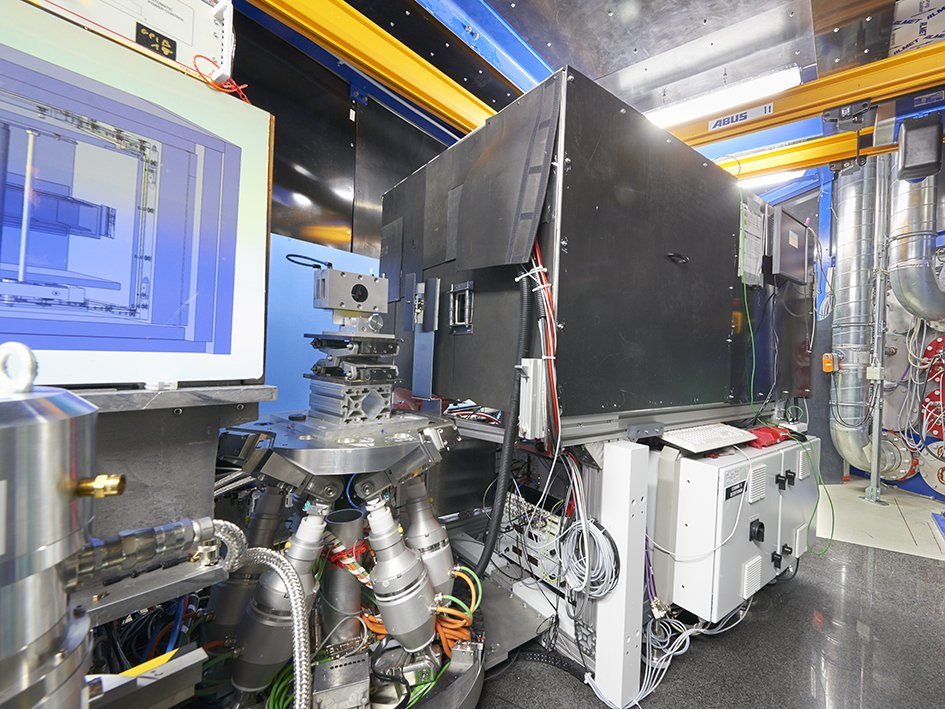
\includegraphics[width=0.7\textwidth]{appendix_instruments_maria}
      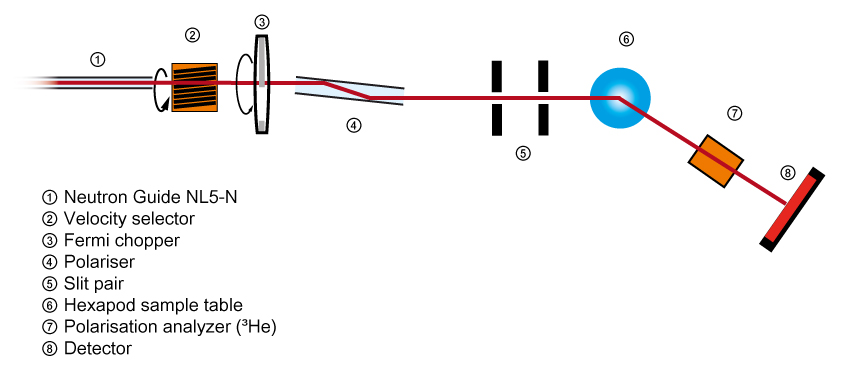
\includegraphics[width=0.7\textwidth]{appendix_instruments_mariaSetup}
      \caption{\label{fig:lss:maria}The MARIA instrument at Heinz Maier-Leibnitz Zentrum used for (polarized) neutron reflectometry and grazing-incidence small-angle neutron scattering (image and schematics reproduced from \cite{Heinz_2015_Maria}).}
    \end{figure}

    The MAgnetic Reflectometer with high Incident Angle (MARIA) at the Heinz Maier-Leibnitz Zentrum is a neutron reflectometer with polarization analysis operated by the J\"ulich Center for Neutron Science (JCNS) \cite{Heinz_2015_Maria}.
    It is designed to study samples with a layer thickness of $0.3 - 30 \unit{nm}$ and can also be used in GISANS mode to study lateral structures on the order of $3 - 300 \unit{nm}$.
    The sample sizes are typically in the order of $10 \times 10 \unit{mm^2}$ and the wavelength of the neutrons can be chosen in a range of $\lambda \eq 4.5 \ldots 10 \angstrom$ for polarized neutrons, with the highest intensity at $4.5 \unit{\angstrom}$.
    To study the magnetic structure of a sample, an electromagnet with up to $1.3 \unit{T}$ is available, as well as a cryostat to cool the sample down to $4 \unit{K}$.

    The sample-to-detector distance in the standard setup is $1.91 \unit{m}$, and the position-sensitive detector has $1024 \times 1024$ pixels with a quadratic dimension of $0.576 \unit{mm}$.
    The sample and collimation apertures for reflectometry experiments are typically set to $2 \unit{mm}$ along the scattering geometry, and the distance in between is $4.1 \unit{m}$.
    This yields an instrumental resolution due to the collimation of approximately $\sigma_q^\mathrm{coll.} \approx 0.01\unit{nm}^{-1}$.
    Additionally, the neutrons have a wavelength spread of $10 \unit{\%}$ (FWHM), which corresponds to an order of magnitude of $\sigma_q^\mathrm{wavel.} \approx 0.04 q$.

    Similar to GALAXI, the neutron reflectometer is controlled onsite by the NICOS software and the data is provided as compressed text files for each detector image and each angle.


\end{document}